%% This is file `elsarticle-template-1-num.tex',
%%
%% Copyright 2009 Elsevier Ltd
%%
%% This file is part of the 'Elsarticle Bundle'.
%% ---------------------------------------------
%%
%% It may be distributed under the conditions of the LaTeX Project Public
%% License, either version 1.2 of this license or (at your option) any
%% later version.  The latest version of this license is in
%%    http://www.latex-project.org/lppl.txt
%% and version 1.2 or later is part of all distributions of LaTeX
%% version 1999/12/01 or later.
%%
%% Template article for Elsevier's document class `elsarticle'
%% with numbered style bibliographic references
%%
%% $Id: elsarticle-template-1-num.tex 149 2009-10-08 05:01:15Z rishi $
%% $URL: http://lenova.river-valley.com/svn/elsbst/trunk/elsarticle-template-1-num.tex $
%%
\documentclass[preprint, authoryear,11pt, 3p]{elsarticle}

%% Use the option review to obtain double line spacing
%% \documentclass[preprint,review,12pt]{elsarticle}

%% Use the options 1p,twocolumn; 3p; 3p,twocolumn; 5p; or 5p,twocolumn
%% for a journal layout:
%% \documentclass[final,1p,times]{elsarticle}
%% \documentclass[final,1p,times,twocolumn]{elsarticle}
%% \documentclass[final,3p,times]{elsarticle}
%% \documentclass[final,3p,times,twocolumn]{elsarticle}
%% \documentclass[final,5p,times]{elsarticle}
%% \documentclass[final,5p,times,twocolumn]{elsarticle}

%% The graphicx package provides the includegraphics command.
\usepackage{graphicx}
\usepackage{subfig}
\usepackage{caption}
%% The amssymb package provides various useful mathematical symbols
\usepackage{amssymb}
%% The amsthm package provides extended theorem environments
%% \usepackage{amsthm}

%% The lineno packages adds line numbers. Start line numbering with
%% \begin{linenumbers}, end it with \end{linenumbers}. Or switch it on
%% for the whole article with \linenumbers after \end{frontmatter}.
\usepackage{lineno}

%% natbib.sty is loaded by default. However, natbib options can be
%% provided with \biboptions{...} command. Following options arehttps://v2.overleaf.com/project/5ae9a183e6e381104e1a8531
%% valid:

%%   round  -  round parentheses are used (default)
%%   square -  square brackets are used   [option]
%%   curly  -  curly braces are used      {option}
%%   angle  -  angle brackets are used    <option>
%%   semicolon  -  multiple citations separated by semi-colon
%%   colon  - same as semicolon, an earlier confusion
%%   comma  -  separated by comma
%%   numbers-  selects numerical citations
%%   super  -  numerical citations as superscripts
%%   sort   -  sorts multiple citations according to order in ref. list
%%   sort&compress   -  like sort, but also compresses numerical citations
%%   compress - compresses without sorting
%%
%% \biboptions{comma,round}

% \biboptions{}

\journal{Socius: Sociological Research for a Dynamic World}

\begin{document}

\begin{frontmatter}

%% Title, authors and addresses

\title{Durable Taste Schemas and Patterns of Cultural Choice}

%% use the tnoteref command within \title for footnotes;
%% use the tnotetext command for the associated footnote;
%% use the fnref command within \author or \address for footnotes;
%% use the fntext command for the associated footnote;
%% use the corref command within \author for corresponding author footnotes;
%% use the cortext command for the associated footnote;
%% use the ead command for the email address,
%% and the form \ead[url] for the home page:
%%
%% \title{Title\tnoteref{label1}}
%% \tnotetext[label1]{}
%% \author{Name\corref{cor1}\fnref{label2}}
%% \ead{email address}
%% \ead[url]{home page}
%% \fntext[label2]{}
%% \cortext[cor1]{}
%% \address{Address\fnref{label3}}
%% \fntext[label3]{}


%% use optional labels to link authors explicitly to addresses:
%% \author[label1,label2]{<author name>}
%% \address[label1]{<address>}
%% \address[label2]{<address>}

%\author[label1]{Omar Lizardo}

%\address[label1]{Department of Sociology, University of California, Los Angeles, 375 Portola Plaza, 264 Haines Hall, Los Angeles, CA, 90095. Email: olizardo@soc.ucla.edu.}

\begin{abstract}
%% Text of abstract
Whether cultural schemas are malleable or durable is a key, but still unresolved, theoretical debate in cultural analysis. In this paper, I contribute to a recent line of work seeking to move this issue to the empirical terrain. To do so, I extract taste schemas from survey data on a representative sample of Americans collected in 2012 containing items on likes and dislikes of musical genres similar to those included in the 1993 General Social Survey culture module. Consistent with the durability position, I find remarkably similar taste schemas in 2012 as those uncovered in the 1993 General Social Survey data in previous work using comparable techniques. Going beyond previous work, I validate these schemas using independent behavioral evidence on musical listening choices and propose a novel way to think about the link between taste schemas and culture consumption behavior that can be generalized to other domains
\end{abstract}

\begin{keyword}
Omnivorousness  \sep Taste \sep Schemas \sep Cultural Choices \sep Univores
%% keywords here, in the form: keyword \sep keyword
%% MSC codes here, in the form: \MSC code \sep code
%% or \MSC[2008] code \sep code (2000 is the default)
\end{keyword}

\end{frontmatter}
\newpage
\section{Introduction}
\subsection{The Durability versus Malleability Debate in Cultural Analysis}
Are cultural schemas durable or malleable? This is a question on which cultural analysts drawing from different theoretical traditions split into different camps \citep{vaisey2016cultural}. One the one hand, we have analysts who talk about schemas as ``deeply internalized'' and ``durable'' cultural elements, and thus as having the potential to show continuity in relation to changes in the external environment \citep{bourdieu1990logic, strauss1997cognitive, patterson2014making}. On the other hand, we have analysts who conceptualize schemas as highly responsive to changes in the external institutional environment and processes, and thus as ``shifting,'' ``multiform'' \citep{dimaggio1997culture, swidler2005anchors, sewell2004concept}. 

Pitched as a theoretical discussion, this debate runs the danger of becoming a purely scholastic issue. Here I break with this approach and instead follow the call recently laid out by \citet{vaisey2016cultural} to move the issue into a more empirical terrain. I use the case of cultural taste schemas to examine the issue of whether we can observe continuity or transformation at the population level over a twenty-year period. The results reveal somewhat remarkable levels of schematic continuity in this domain, a pattern consistent with the relative durability thesis \citep{vaisey2016cultural}. However, partially consistent with the malleability position, the differences that we do observe can be readily traced to institutional transformations on the consumer and production side of musical genres, such as the aging of the Rock and Roll generation and the emergence of hip-hop and rap as a prototypical ``pop'' or ``industry'' genre. 
\subsection{The Case of Cultural Taste Schemas}

Cultural taste schemas, especially those linked to the underlying association shared by people with respect to musical genre categories, represent a strategic research site with which to address the issue of schematic durability. This is for two reasons. First, both theoretical and methodological developments with regard to extraction of latent schemas from observed responses in survey data have used this case, and the associated data source (the 1993 General Social Survey), as their primary testbed \citep{goldberg2011mapping, boutyline2017improving}. This means that we have a set of relatively well-established results documenting population-level variability on taste schemas in the American public at this time characterizing the nature of each evaluative schema, thus facilitating comparison. 

Second, the domain of musical taste is different from other institutional settings such as politics. In the political domain, we might expect continuity and durability in people's conceptions to be fixed by the relative durability of external institutional arrangements (e.g. the two-party system in the U.S.). And in fact, this is precisely what we observe. In a landmark study, \citet{baldassarri2014neither} find remarkable continuity in the ways Americans organize their understanding of political issues at the population level across twenty years (although they could not engage in apples to apples comparisons of the same items as we do here). A durability theorist might see this as strong evidence for their position, but a malleability theorist could point to continuity (even with change at the margins) in external institutional arrangements as a competing explanation. In the case of politics, therefore, continuity seems over-determined by external and internal mechanisms, making it hard to adjudicate between the durability and malleability positions. 

Musical taste, by way of contrast, represents a case in which radical transformations have occurred in terms of production, distribution, modes of consumption, as well as definitions of genre popularity and ``aesthetic mobility'' \citep{baumann2001intellectualization} since the early 1990s. Thus, if we were to expect, consistent with the malleability thesis, that schemas respond to radical structural and external changes in a given domain, then the domain of musical evaluation would be an ideal case in which to observe such transformations. On the other hand, observing relative continuity in this domain would support a strong version of the durability thesis \citep{vaisey2016cultural}. In this paper, I set out to do just that by analyzing twenty distinct musical genres—ranging from Classical and Opera to Rap and Heavy Metal—to see how they cluster together in people's minds. Specifically, I anticipate that core anchors like Rock, Pop, and Rap will fundamentally organize taste schemas, while others like Heavy Metal will remain polarized. 

\subsection{Terminology and Approach}
It is important to get clear on the use of certain specialized terms that will recur through the manuscript. In what follows, I refer to the latent schema presumed to be responsible for a given pattern of observed responses to evaluative questions in a cultural taste survey as a \emph{taste schema}. Persons who share the same (or similar) latent taste schemas are members of a \emph{schematic class}. Following \citep{boutyline2017improving}, I refer to \emph{schematic class analysis}, as a set of procedures designed to classify respondents based based on their sharing latent schemas governing their observed (usually evaluative) ordered responses to a given set of objects in survey data (such as likes and dislikes of musical genres in the case of cultural taste). 

Traditional methods such as factor analysis, latent class analysis, or principal component analysis attempt to group respondents into classes based on differences in their observed responses. The assumption is that there is a one-to-one correspondences between latent constructs driving the responses (such as an attitude) and observed response patterns. Persons at the same level (or in the same category) of the latent construct will produce similar observed responses. Schematic class analysis, by contrast, exploits the distinction between a latent schema, which is an unobserved pattern of associations as to what goes with what or what is the oppossite of what, and an evaluation which is a ``pro'' or ``con'' (or in mixed) attitude directed to an object \citep{goldberg2018beyond}. Two people can agree about the way they think two objects are associated (e.g. thinking that Classical music is completely opposed to Country music), while being at different ends of the evaluative scale with respect to the same pair of objects (one person loves Classical and hates Country, while the other is a Country fan who thinks Classical is boring). 

The above implies that persons can provide different observed evaluative response patterns even when they share the same latent schema with regard to the relation between a set of objects. The goal of schematic class analysis is thus to partition respondents based on these latent schemas exploiting specifiable relations between observed response patterns. \citet{boutyline2017improving} argues that this can be done under the assumption that, when two different observed response patterns come from the same schema, the two response sets will be related via a finite set of transformations, such as inversion or rescaling (or both).

{\em Correlational Class Analysis} (CCA) is a variant of schematic class analysis that uses the absolute value of the Pearson correlation coefficient between the response vectors of different respondents as a schematic similarity criterion. The idea being that the observed response patterns of two people have a large absolute correlation, they are likely to have been produced by transformations of the same latent schema \citep{boutyline2017improving}. Like relational class analysis, CCA partitions the resulting (weighted) network of respondents, where links are based on the absolute value of the correlation, using a modularity maximization algorithm. \citet{boutyline2017improving} shows that the correlation approach outperforms other ways of computing response pattern similarity, and thus eliciting schematic class membership, such as Goldberg's \citeyear{goldberg2011mapping} use of the ``relationality'' measure in relational class analysis. Given this, I use correlational class analysis as the main approach to extracting schematic classes in what follows.  

\subsection{Previous Work Using Schematic Class Analysis}
Schematic class analysis, whether based on relationality or the correlation distance, has been used in a variety of applications to extract schematic classes from mass survey responses. These include political belief logics \citep{baldassarri2014neither, daenekindt2017people}, patterns of thought about the markets and the economy \citep{dimaggio2018searching, metzmcDonnell2018multiple}, and taste schemas about the link between science and religion \citep{dimaggio2017culture}. In addition, recent work by \citet{daenekindt2017structure} analyzes the structure of aesthetic dispositions among a sample of museum-goers, a topic close to that dealt with here. In this respect, schematic class analysis has already made major contributions to the social science literature across a wide range of topics. 

\subsection{Contributions of the Present Work}
Previous work using schematic class analysis suffers from validation limitations. In particular, previous studies are forced to rely on inspecting differences in the correlations between items within classes (internal validation) or the correlation between schematic class membership and demographic characteristics to both validate schematic class assignment, and make inferences about the possible effect of schemas on behavior. \citet{goldberg2011mapping} used internal, and demographic validation strategy in the original study using 1993 General Social Survey data.\citet{baldassarri2014neither} used a combination of internal, demographic, and criterion-based strategies (looking at how predictors differ in predicting partisanship across schematic classes). In a similar way \citet{dimaggio2018searching} and \citet{dimaggio2017culture} use a combination of internal, demographic, and substantive validation strategies.\footnote{Note that this discussion is not related to validation of the \emph{number} of classes extracted by schematic class analysis methods such as RCA or CCA. In this respect, \citet{boutyline2017improving} have used multiple group SEM, and \citet{dimaggio2017culture} and \citet{dimaggio2018searching} have used network randomization methods coupled with cluster validation (e.g. gap statistic) techniques.}

This study adds to and extends previous work by using both the standard internal validation approach (based on within-class inter-item correlations) and also behavioral (or criterion) validation using a measure of choice behavior directly related to the domain in question, namely, music listening habits. In this respect, my strategy comes closest to the that pursued by \citet{baldassarri2014neither}. This allows me to determine empirically the behavioral potential of schematic classes in a way that establishes external (predictive) validity within the musical taste domain. I incorporate insights from recent work in the analysis of item correlation networks \citep{epskamp2012qgraph}, and link recently developed formal measures of item position in the taste schema with behavioral predictive criteria. Promising results obtained with this approach recommend it as a useful strategy for future schematic class analysis work. 

\section{Data and Variables}
In the summer of 2012, I fielded a survey that was (partially) designed to replicate the General Social Survey 1993 Culture Module. This last is now a canonical dataset, providing the empirical basis for large and variegated set of analyses (and re-analyses) in the sociology of taste \citep[][among others]{boutyline2017improving, bryson1996anything,bryson1997univores, goldberg2011mapping, han2003unraveling, okada2017structure, tampubolon2008revisiting}. It can be said without exaggeration that the bulk of our knowledge of the cultural taste patterns of the American population, both in terms of schematic form and actual content, are due to this data source. As such, the addition of a more contemporary source on the musical taste patterns of the American population constitutes a valuable addition on its own right \citep{lizardo2016cultural, lizardo2016end, lizardo2015musical}.

The data used in this paper were collected by Survey Sample International (SSI), a private firm that specializes in sampling, data collection, and analysis. SSI managed recruitment and participation invitation tasks to generate a panel of adults from which our working sample was drawn. Survey respondents were selected from the panel for participation on the basis of age, gender, race, education, and geographic region to approximate a sample representative of the U.S. population, $N = 2,250$.

Like General Social Survey 1993, SSI 2012 included items assessing respondents’ likes and dislikes (as well as a middle category of ``mixed feelings'') for 20 categories of musical style: (1) classical or symphony and chamber, (2) opera or operetta, (3) jazz, (4) Broadway musicals or show tunes, (5) mood or easy listening, (6) big band or swing, (7) classic rock or oldies, (8) country, (9) bluegrass, (10) folk, (11) hymns or gospel, (12) Latin or Spanish/salsa, (13) rap or hip hop, (14) blues or R and B, (15) reggae, (16) top 40 or pop music, (17) contemporary rock, (18) indie or alternative rock, (19) dance or club/electronic, and (20) hard rock or heavy metal. These responses are the basis of the schematic class analysis. 

The survey also asked respondents to report in a separate item whether they regularly {\em listen} to each one of the genres listed. Responses to these items allow us to examine behavioral expression (and variation) across schematic classes separately from the items used to elicit schematic class membership.

\section{Correlational Class Analysis}
I follow the same data analysis procedure as \citet{boutyline2017improving}, with two modifications. The first is relatively minor; given the nature of the taste evaluation items as limited ordinal response items, I use the polychoric correlation coefficient as a ``drop-in replacement'' \citep[386]{boutyline2017improving} for the Pearson correlation.\footnote{Polychoric correlations were computed using the function \texttt{cor\_auto} of version 1.5 of the \texttt{R} package \texttt{qgraph} \citep{epskamp2012qgraph}.}

The second is less trivial and has to do with the way I treated the ``not familiar with this genre" responses to genre evaluation questions.  \citet{goldberg2011mapping} recoded these to the ``mixed feelings'' (middle) response for all respondents who offered this response for six genres or less (dropping those who were not familiar with seven or more genres). \citet{boutyline2017improving} followed this same coding strategy for purposes of strict replication. 

Since ``not familiar" responses are a type of missing data, I follow recently recommended best practice and use multiple imputation rather than fixed value recoding. This strategy is more efficient and does not require us to choose an arbitrary cutoff to decided how many ``not familar" responses are sufficient to drop a respondent from the analysis. The variables used in the multiple imputation procedure consisted of the other genres for which the respondent did provide a valid taste response. To avoid issues with median aggregation across multiple imputations, I utilized a single robust imputation via predictive mean matching. This was performed using the \texttt{mice} package in \texttt{R}, generating a complete dataset for the correlational class analysis without creating artificial fractional ordinal values. The distribution of ``not familiar'' responses is highly skewed: $1,511 (67\%)$ of respondents claimed to be familiar with all genres; another $11\%$ reported only one ``not familiar'' response. By the time we get to six ``not familiar'' responses we have reached $95\%$ of respondents. Thus, only 5\% of the analytic sample contains seven or more imputed responses. After dropping respondents who did not provide taste responses on any of the 20 genres ($N = 21$) and dropping respondents who provided the same response across all genres ($N = 72$), which correlational class analysis would treat as its own ``degenerate'' schematic class, the final analytic sample is $N= 2,183$.

\subsection{Correlation Networks for Schema Extraction} 
As is now standard, I present the resulting schematic classes as correlation networks \citep{ boutyline2017improving, goldberg2011mapping, epskamp2012qgraph}, with the edge weight set to the estimated correlation for each genre pair for members of that class and the node color set to the assignment of each genre to one of four latent factors based on the binary consumption items (results from which are shown in figure~\ref{fig:typology}). Correlation networks for each taste schema are shown in Figure~\ref{fig:corrnet} (Top). 

\subsubsection{Expected Influence Score}
To quantify the importance of the evaluation of different genres within each class, I follow the approach recommended by \citet{robinaugh2016identifying} for analyzing node centrality in signed correlation networks and rank each genre in each taste schema by its \emph{expected influence}. Fundamentally, Expected Influence is a form of weighted degree centrality \citep{barrat2004architecture}, given by:

\begin{equation}
EI_{gs} = \sum_{j=1}^{N} r_{gjs}    
\end{equation}

Where $EI_{gs}$ is the expected influence of the $g^{th}$ genre in the $s^{th}$ taste schema and $r_{gjs}$ is the value of the polychoric correlation coefficient between the taste evaluations for genre $g$ and genre $j$ among respondents who share taste schema $s$. Following Robinaugh et al. (2016), we can interpret this metric through the lens of a ``spreading activation'' model. In this framework, an increase in the evaluation of a focal node probabilistically causes an increase in positively tied nodes and a decrease in negatively tied nodes. Therefore, genres with the highest $EI$ (those with strong, positive ties to many other genres) are expected to exert the most structural ``influence'' over the state of the overall network. To facilitate direct comparison across schemas, centrality measures are standardized to Z-scores. Figure~\ref{fig:corrnet} (Bottom) shows the rank of each genre according to $EI_g$ for each taste schema.\footnote{$EI_g$ is computed using the \texttt{expectedINF} function included the \texttt{R} package \texttt{networktools} \citep{networktools}.}

\section{Results}
\subsection{Number of Taste Schemas and Class Sizes} 
Subjecting the data to CCA, yields a solution (setting weights in the respondent by respondent correlation network below $p<0.01$ to zero) that partitions the sample into five schematic classes.\footnote{To perform correlational class analysis, I used the routines included in the \texttt{R} package \texttt{corclass} \citep{corclass}.} This is similar to the results reported in \citet{boutyline2017improving} applying the same method to General Social Survey data, who found four schematic classes characterizing the American population in 1993. The classes that I obtain using the SSI 2012 data are somewhat uneven in size, with $N = 481 (22\%), 369 (17\%), 574 (26\%), 419 (19\%),$ and 340 (16\%) respectively. 
      
\subsection{Schema Interpretations}
Based on the psychometric network structures and node centralities, we can interpret these schematic classes not just by \emph{what} respondents like or dislike, but by how their tastes are \emph{organized}. Genres with high \textbf{Strength} act as core anchors---meaning feelings about that genre strongly dictate feelings about the rest of the music landscape. \textbf{Betweenness} highlights genres that act as bridges connecting disparate clusters.

\begin{itemize}
\item \textbf{Schema 1: The ``Highbrow / Rock Anchor'' Schema.} Core Anchors: Classical, Contemporary Rock, Classic Rock, Jazz. For this group, ``highbrow'' genres and standard rock act as the central organizing principles. Their opinions on these genres strongly predict their entire taste profile. They tend to strongly reject Rap and Opera.
\item \textbf{Schema 2: The ``Classic Rock / Pop Core'' Schema.} Core Anchors: Classic Rock, Rap, Bluegrass. This schema represents a very common taste profile anchored centrally by Classic Rock. Interestingly, Rap has very high strength and betweenness here---meaning that whether they tolerate or reject Rap is a massive polarizing divider that structurally dictates the rest of their network.
\item \textbf{Schema 3: The ``Pop / Contemporary Bridge'' Schema.} Core Anchors: Pop, Contemporary Rock, Opera, Rap. Organized heavily around mainstream pop and contemporary music, Pop is the absolute central load-bearing pillar. Opera acts as a strong negative anchor (highly central because almost everyone in this class uses their uniform dislike of it to structurally define their taste).
\item \textbf{Schema 4: The ``Easy Listening / Roots'' Schema.} Core Anchors: Easy Listening, Pop, Bluegrass, Jazz. A softer, traditionalist schema. Harder genres like Heavy Metal are pushed completely to the network's periphery. The network revolves structurally around accessible, easy-to-digest music and roots music.
\item \textbf{Schema 5: The ``Polarized / Omnivore'' Schema.} Core Anchors: Rap, Big Band, Contemporary Rock, Folk. The most eclectic and structurally diverse schema. The core anchors span across completely different historical and cultural eras. High betweenness for these genres means this class evaluates music across boundaries, heavily indicating an ``Omnivore'' profile where genres serve as bridges rather than isolated islands.
\end{itemize}

\subsection{Behavioral Validation of Taste Schemas Using Music Listening Choices}
As noted earlier, previous work using schematic class analysis generally lacks a behavioral criterion with which to validate results. Analysts usually have to rely on indirect validation procedures, such as looking at the correlation between taste schemas and demographics \citep{goldberg2011mapping, baldassarri2014neither} and inferring subsequent behavior from what is known about the correlation between demographics and action. The 2012 survey asked respondents to not only evaluate genres but also to list whether they listened to those genres or not. This information provides a source of behavioral validation for the schematic classes. 

\subsection{Centrality in a Taste Schema Predicts the Link Between Omnivorousness and Evaluation}
More convincing evidence for the criterion validation of the schematic classes would be to link the position of each genre in the schematic network to cultural consumption as a behavioral criterion. 

The validation strategy here adapts the design used by \citet{robinaugh2016identifying}. In their work, Robinaugh et al. first used simulations of a ``spreading activation'' model to demonstrate that the Expected Influence ($EI$) of a node correctly predicts how much effect its change in activation would have on the rest of the network. They then empirically validated this by showing that a node's $EI$ tracked its behavioral predictiveness over time. Adapting this logic to cross-sectional data, we can define a behavioral measure of importance for genre $j$, $importance_j$, as the correlation between a respondent's evaluation of genre $j$ and their overall behavioral omnivorousness (the total count of genres they actually listen to). If the spreading activation model holds as a useful methodological heuristic, the structural centrality of a genre ($EI_j$) should track this behavioral measure of importance. 

Now imagine, the same process but this time we ``activate'' (by producing a positive evaluation) a genre that is peripheral in the correlation network of that schema (like Country or Hip Hop in Figure~\ref{fig:corrnet}). Because such genres feature mostly null or negative links with other musical styles, then we should expect that the evaluation of those genres should be decoupled (or in the case of negative correlations lead to a devaluation) of the other genres in the schema. In this case, there is no spreading activation and no empirical expectation that evaluations of these genres should be linked to behavioral omnivorousness. 

Because evaluation is usually strongly linked to consumption behavior, then liking lots of genres should result in an increased likelihood of actually listening to a lot of musical styles under normal conditions (displaying omnivorousness  in consumption behavior), and liking only a few should make you a univore. 

If this imagery of the way taste schemas link to behavior is on the right track, then we should expect that omnivorousness should be positively correlated with the positive evaluation of the {\em most central genres} in each taste schema. In the same way, the number of genres actually listened to should have a lower correlation with the evaluation of genres that are peripheral in the correlation network for that schema. This is a cognitively plausible, and empirically verifiable, way of conceptualizing the link between taste schemas and consumption behavior, and one that should obtain if schemas are a valid predictor of such behavior. 

Results of an analysis meant to evaluate this hypothesis are shown in Figure~\ref{fig:money}. In the figure the y-axis gives the Spearman rank correlation between an indicator of behavioral omnivorousess---number of genres that people who share that schema listen to---and the ordinal taste evaluation item for that genre (higher values coded as liking that genre), re-scaled to the variance for that taste schema. The x-axis is the importance of the genre in the corresponding taste correlation network (as given by the expected influence ($EI_{gs}$) score; see figure~\ref{fig:corrnet}). 

As expected, we see a positive correlation between these two quantities within all five taste schemas, with the correlation being strongest ($r = 0.68$) for the omnivore/univore schema. The upper-right of each scatterplot shows those genres for which there is a stronger than expected correlation between choosing a lot of genres and actually liking that genre. This in effect, gives us the expected taste profile for the omnivores in each class, in effect providing a schematic basis for the claim, now fairly standard in the sociology of taste, that there are multiple ``varieties'' of omnivorousness at the level of consumption \citep{coulangeon2015social, ollivier2008modes, savage2011unravelling}. 

Thus, Schema 1 (Highbrow/Rock Anchor) omnivores are expected to combine Classical, Contemporary Rock, and Jazz; Schema 2 (Classic Rock/Pop Core) omnivores should be more likely to combine Classic Rock, Bluegrass, and Rap; Schema 3 (Pop/Contemporary Bridge) omnivores are expected to listen to Pop, Contemporary Rock, and Rap; Schema 4 (Easy Listening/Roots) omnivores like Easy Listening, Pop, Bluegrass, and Jazz; finally, Schema 5 (Polarized/Omnivore) omnivores are mostly attracted to an eclectic variety of genres, such as Rap, Big Band, Contemporary Rock, and Folk. This constitutes suggestive evidence for the behavioral validity of the correlation networks extracted from each taste schema and the spreading activation interpretation of the link between the resulting schemas and patterns of cultural choice. 

The lower-left quadrant of each scatterplot shows genres for which there is a lower than expected correlation between behavioral omnivorousness and the evaluations of genres that are peripheral to each taste schema. This in effect, gives us the expected consumption profile of \emph{univores} in each schema, providing evidence for the oppositional characterization of the nature of each schemas extracted from the correlation networks. 

\section{Discussion and Conclusion}
This paper began with the debate over the malleability versus the durability of schemas in cultural analysis. To shed empirical light on this issue, I revisited the relatively well-studied issue of heterogeneity in evaluative schemas for musical genres in the American population \citep{goldberg2011mapping}. Using recently collected survey data comparable to the General Social Survey 1993 culture module, I find that taste schemas of Americans in 2012, bear a strong resemblance from those uncovered in previous work using comparable techniques (most closely \citet{boutyline2017improving}). I interpret these results as providing strong evidence that, at least at the population level, there is strong continuity and durability in the way Americans organize their understandings of an important cultural domain. These findings deepen and extend recent arguments arguing against extreme versions of the schematic malleability thesis, showing that we find relatively strong levels of population-level durability in a variety of cultural patterns \citep{vaisey2016cultural}. At the same time, the minor structural shifts observed in 2012—such as the repositioning of Hip Hop/Rap as a highly central organizing anchor in certain schemas, and the migration of Jazz toward traditionalism—highlight that schemas are not entirely static. Instead, they exhibit bounded malleability, adapting to macro-level institutional transformations in music production and consumption without losing their core structural integrity.

This paper also contributes and extends previous work in survey-based schematic class analysis by attempting to validate the results of the resulting schema partitions using behavioral criteria linked to the domain in question (in this case, patterns of musical listening choices). Building on the work of \citet{goldberg2011mapping}, who utilized network metrics like the clustering coefficient to examine schema networks, I showed that we can leverage modern techniques developed for Exploratory Graph Analysis (using the Leiden algorithm) to go beyond eyeballing \citep{epskamp2012qgraph,networktools}. In particular, I showed that a simple measure of vertex centrality referred to as ``expected influence'' \citep{robinaugh2016identifying}, does a good job of capturing the genres most central in each schema. The validation results reveal two sets of notable findings. 

I found that the taste schema featuring the lowest number of negative links among evaluative items (labeled Omnivore-Univore in previous work) is indeed the most omnivorous in terms of their actual likelihood to listen to a wide variety of musical styles. This supports the idea that at least in some cases, behavioral predictions can be made from ``eyeballing'' the correlational network corresponding to a given schema. However, beyond these broad predictions, it is perilous to conflate the evaluative structure of a schema with its behavioral potential. For instance, I find that all taste schemas have potential for a form of omnivorousness, but this cannot be ascertained from a global assessment of the correlation structure. Instead, the relative importance of genres within the schema must be linked to behavioral outcomes in question. 

Following this approach, I showed that influential genres in the correlation network are also those for which there is a strong correlation between omnivorousness (in terms of actual choice behavior) and positive evaluation. I argued that this pattern of results can be accounted for if we read the schema correlation as a possible conduit for ``spreading activation'' of evaluations. This allows us to pick the genres the evaluation of which will be strongly coupled to the evaluation of other genres in the schema, from those whose evaluation will be loosely coupled. The within-schema correlation between omnivorousness at the level of consumption choices and the taste evaluation of each can then be used to define distinct omnivore/univore profiles for each class, thus providing schematic foundations for the claim that there are ``varieties'' of omnivorousness (and univorousness).

Despite these promising results, several limitations should be noted. Because the behavioral listening measures and the taste evaluations are self-reported concurrently in a cross-sectional design, we cannot rule out consistency bias—where respondents who express a liking for a genre are also more likely to report listening to it simply to maintain self-consistency. Consequently, these findings should be interpreted with care, and the ``spreading activation'' model should be understood as a useful methodological heuristic rather than a literal causal diagram of taste formation. Future longitudinal work would be necessary to establish a direct causal link between changes in schema organization and subsequent music consumption behavior. 

\newpage
\section*{References}
\bibliographystyle{elsarticle-harv}
\bibliography{main.bib}
\newpage

%Factor analysis of consumption items
\begin{figure}[t!]
\centering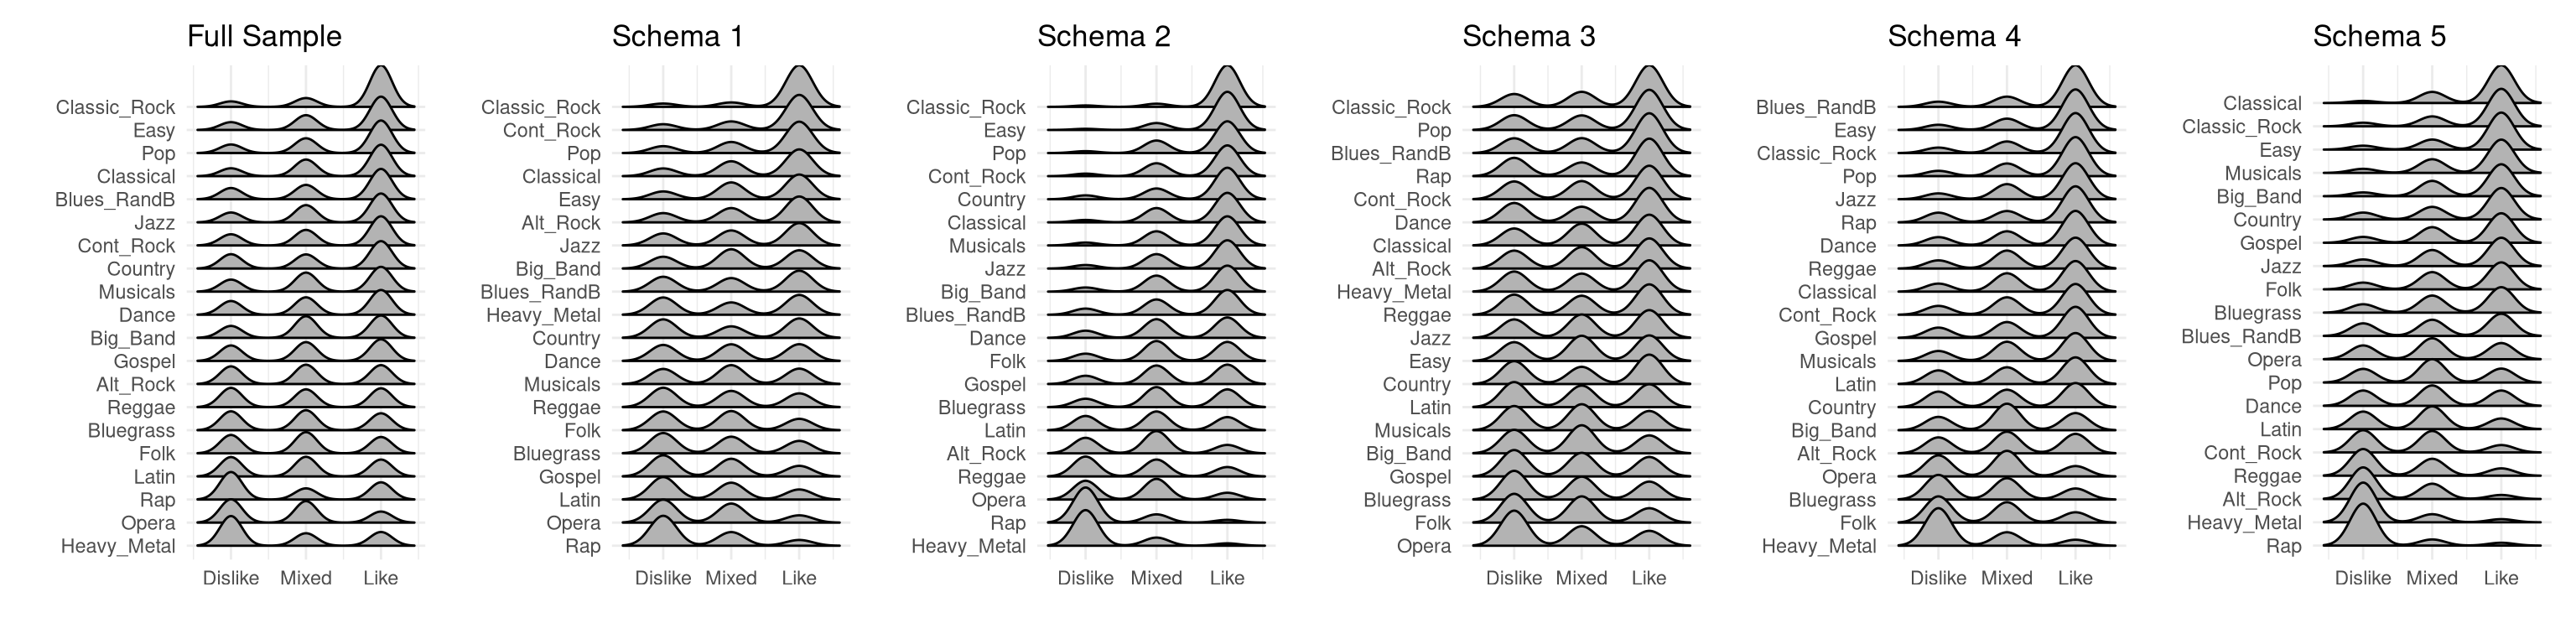
\includegraphics[width=1.0\linewidth]{qmd/main-analysis_files/figure-html/ridge-plots-1.png}
\caption{\scriptsize Genre Evaluations by Schematic Class. The plots display density ridges for the evaluations of each genre across the five uncovered taste schemas.}
\label{fig:typology}
\end{figure}

%comparing standard and LASSO regularized correlation networks (node-link diagrams)
\newpage
\begin{figure}[ht!]
  \centering
  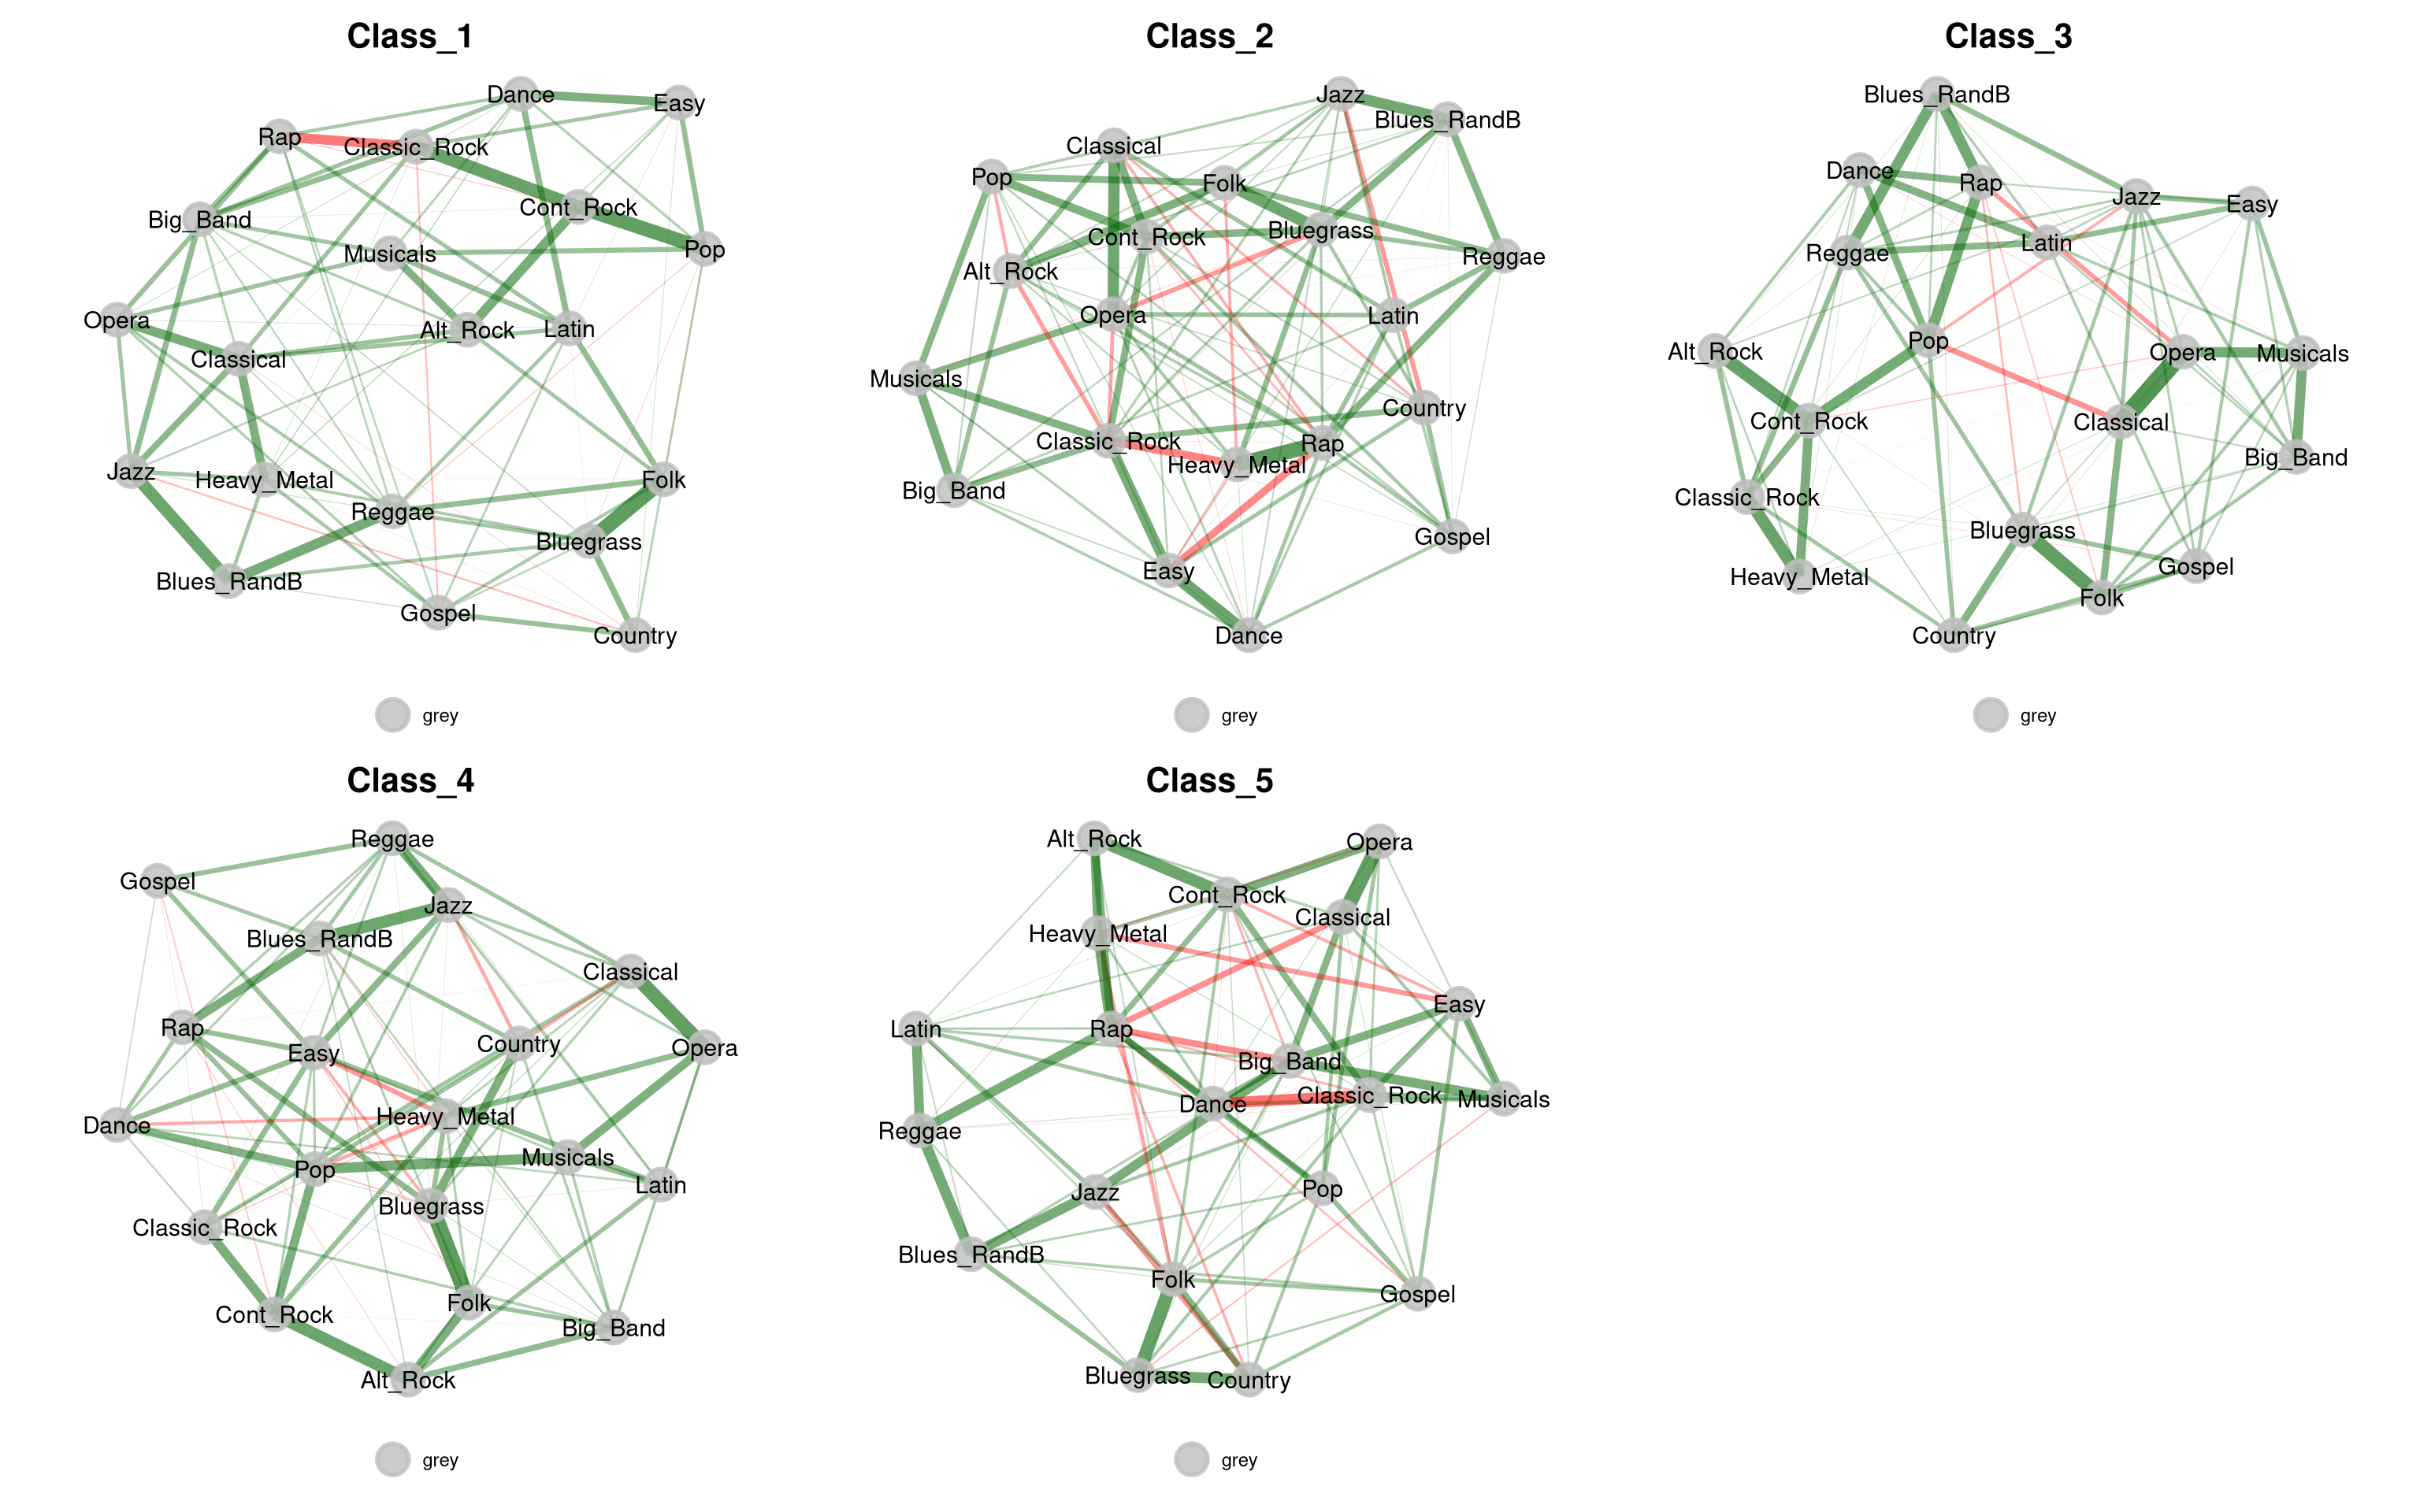
\includegraphics[width=1.0\textwidth]{qmd/main-analysis_files/figure-html/network-plots-1.png} \\
  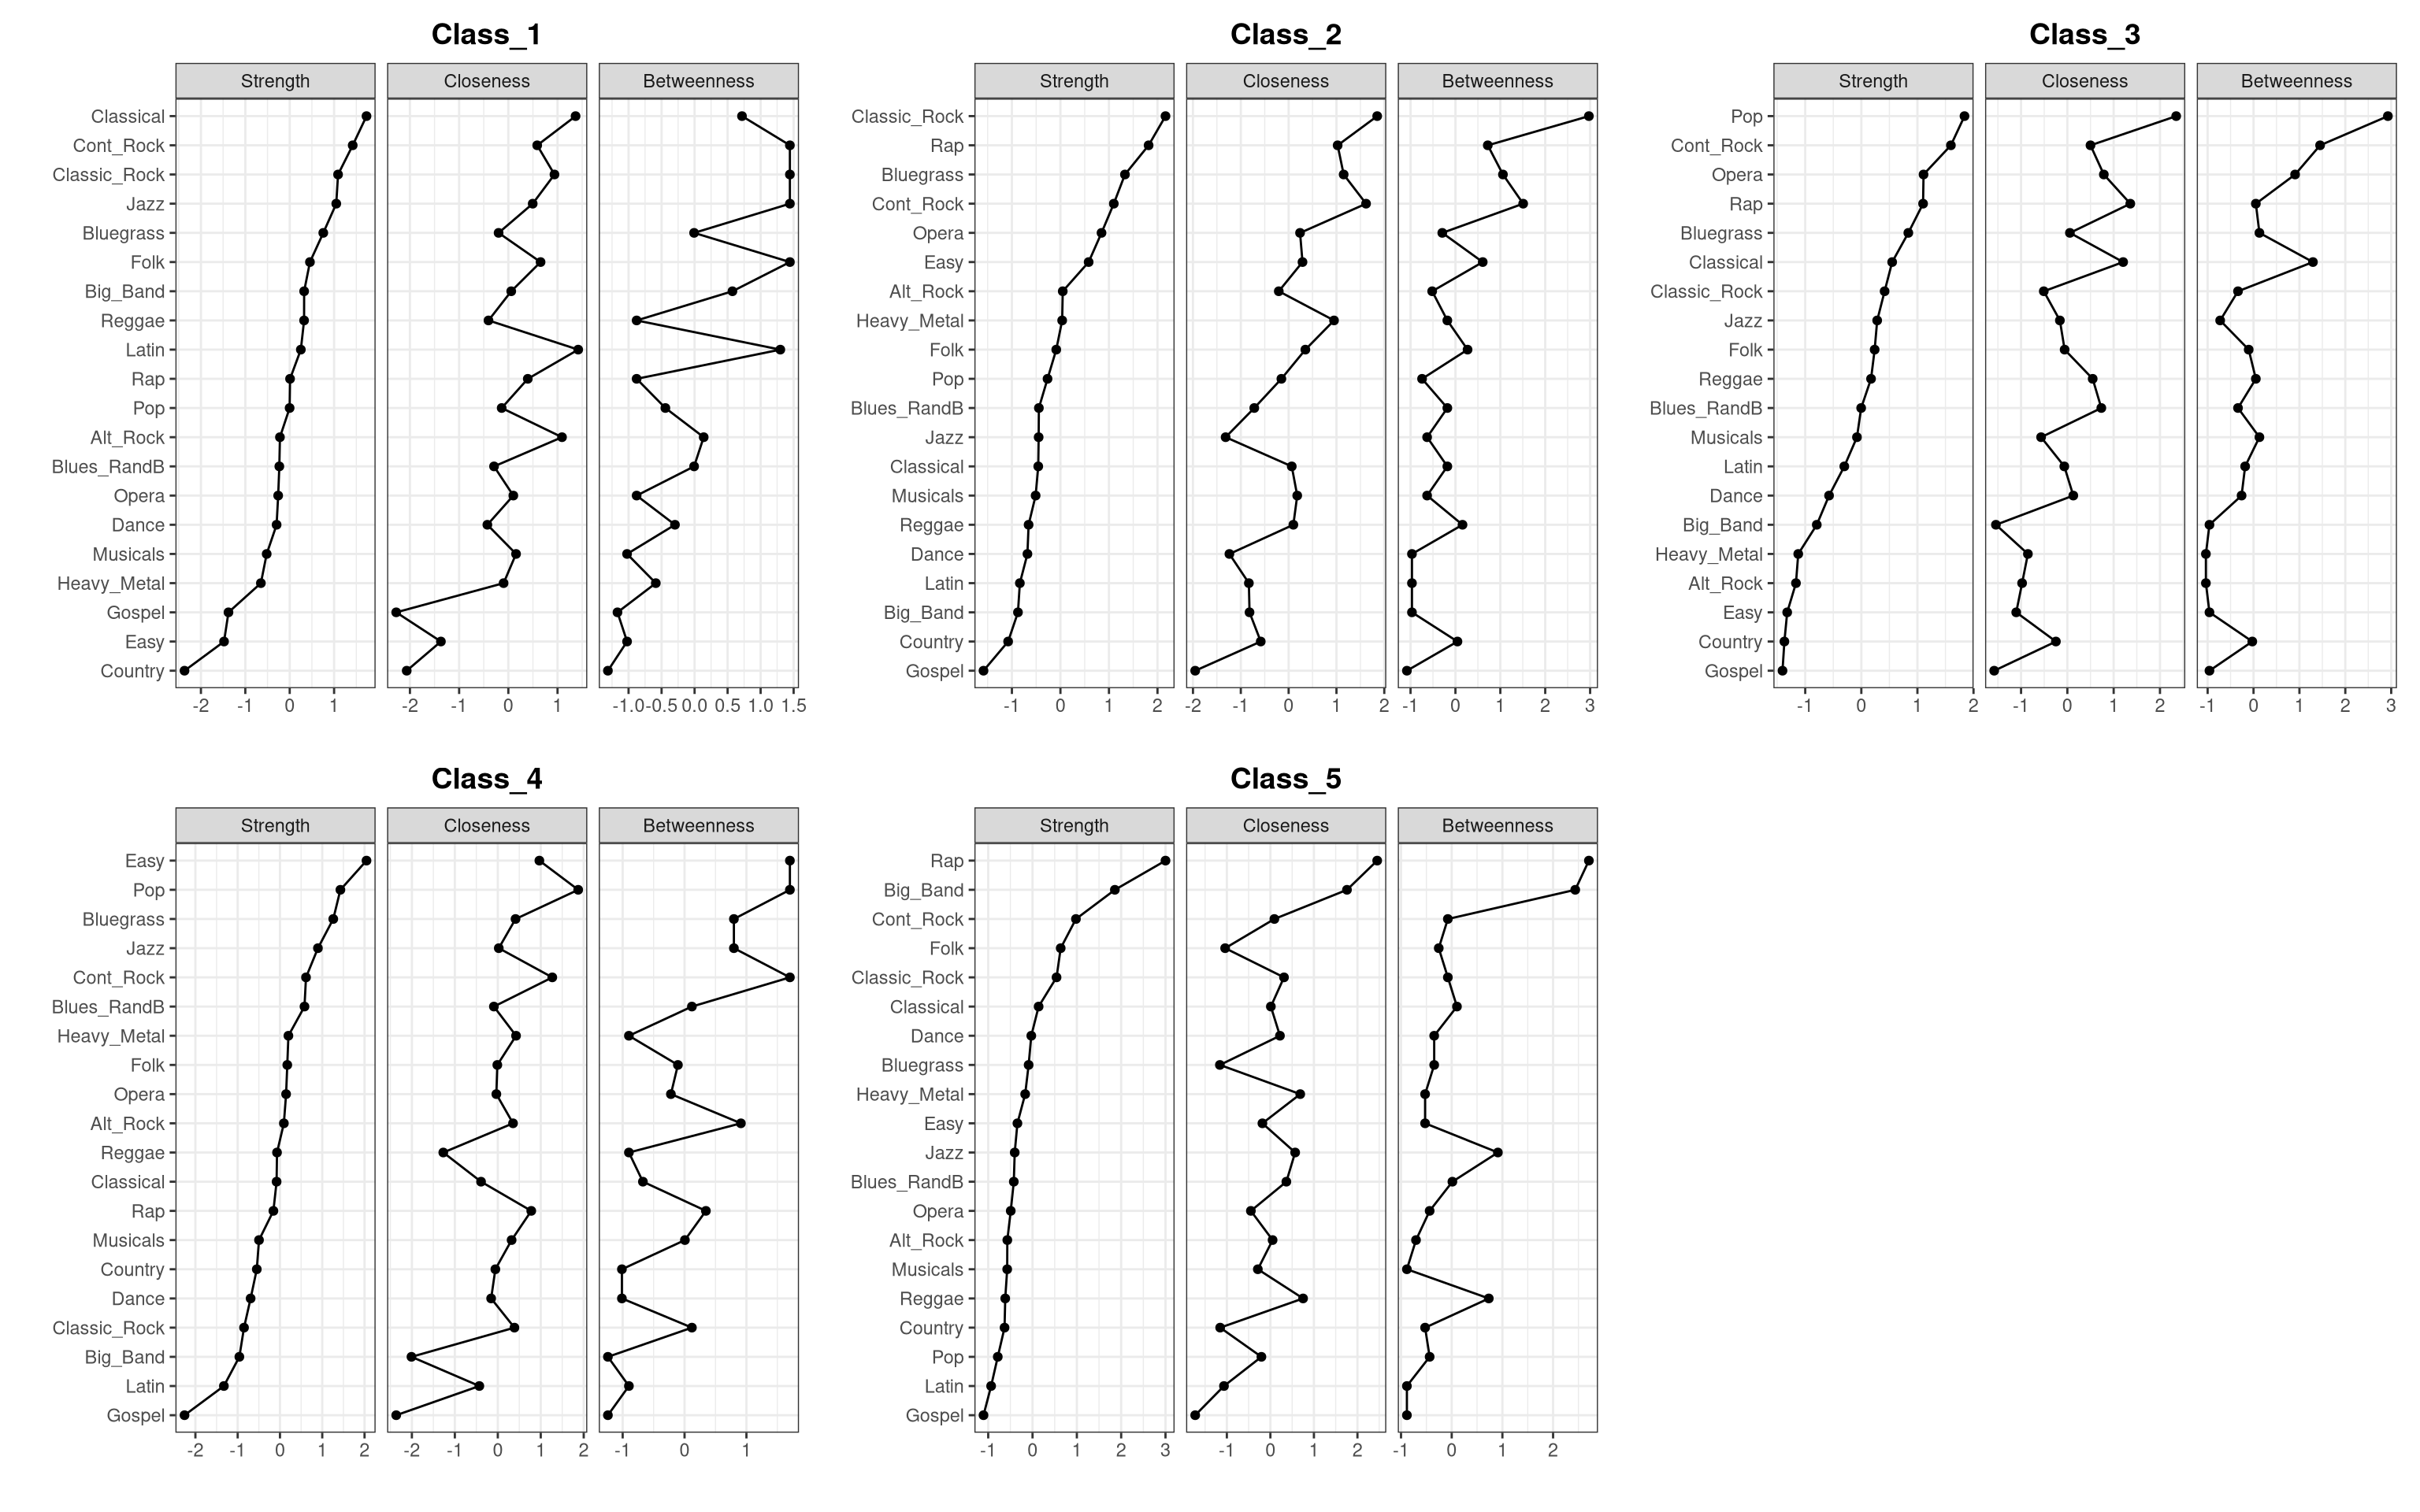
\includegraphics[width=1.0\textwidth]{qmd/main-analysis_files/figure-html/centrality-plots-6.png}
  \caption{\scriptsize \newline \textbf{Top:} Correlation Networks for each taste schema estimated via EGA. Nodes are grouped based on the communities identified by the Leiden algorithm. \newline \textbf{Bottom:} Standardized centrality measures (Strength, Closeness, and Betweenness) for each genre within each taste schema, ordered by Strength.} 
  \label{fig:corrnet}
 \end{figure}
    
 %N. of Genres by Schematic Class
 \newpage
\begin{figure}[ht!]
  \centering
    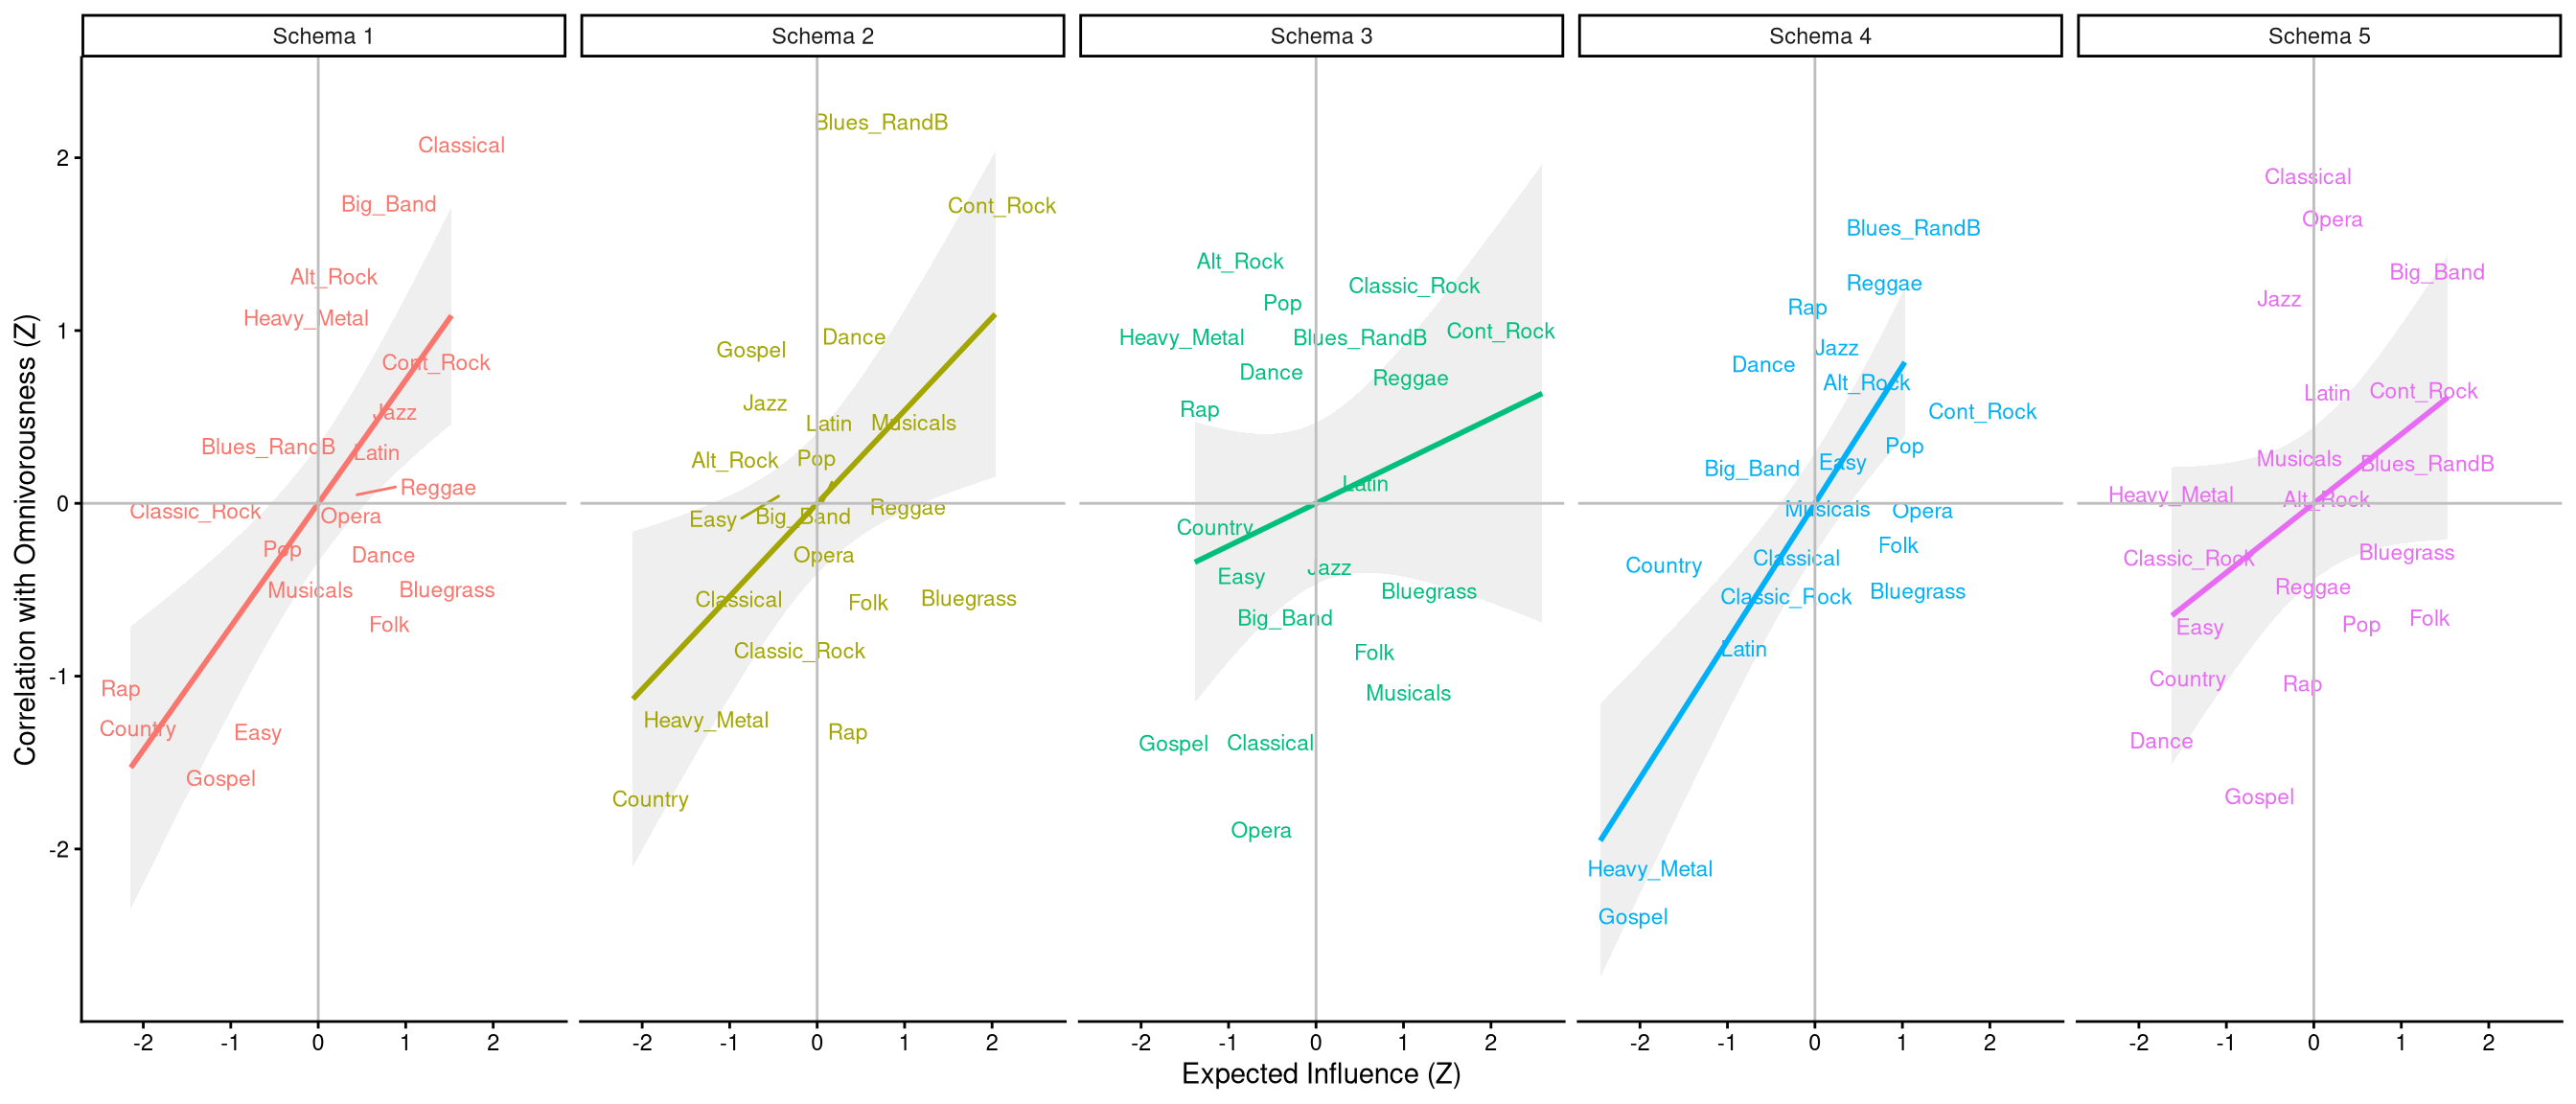
\includegraphics[width = 1.0\textwidth]{qmd/main-analysis_files/figure-html/validation-step-1.png}
    \caption{\scriptsize \newline Y-axis is the (rescaled within taste schema) Spearman rank correlation between number of genres respondents listen to and their taste evaluation of that genre (higher values indicating the respondent likes the genre). X-axis is the (standardized at taste schema class mean) expected influence ($EI_{gs}$) of that genre in the correlation network for that schema. Within each taste schema, the positive correlation between omnivorousness and evaluation tends to increase as the centrality of that genre in the schema goes up.}
  \label{fig:money}
 \end{figure}
 
%% Authors are advised to submit their bibtex database files. They are
%% requested to list a bibtex style file in the manuscript if they do
%% not want to use model1-num-names.bst.

%% References without bibTeX database:

% \begin{thebibliography}{00}

%% \bibitem must have the following form:
%%   \bibitem{key}...
%%

% \bibitem{}

% \end{thebibliography

\end{document}

%%
%% End of file `elsarticle-template-1-num.tex'.